\documentclass[../report.tex]{subfiles}

\begin{document}
Vi xử lý 8086 là phiên bản nâng cấp của vi xử lý 8085 được phát triển từ năm 1976. 
Nó là vi xử lý 16 bit, có một tập lệnh mạnh mẽ và cung cấp phép toán nhân, chia trực tiếp trên phần cứng. 
Bao gồm 20 chân địa chỉ và 16 chân dữ liệu. 
Do đó nó có thể truy cập tới 1MB bộ nhớ. 

Nó có 2 chế độ hoạt động là chế độ Maximum và chế độ Minimum. Chế độ Maximum phù hợp với hệ thống có nhiều 
vi xử lý và ngược lại chế độ Minimum phù hợp với hệ thống chỉ có một vi xử lý. Ở đây ta chỉ quan tâm tới chế 
độ Minimum. 

Những đặc điểm nổi bật của vi xử lý 8086: 
\begin{itemize}
    \item Nó có hàng đợi lệnh, cho phép lưu trữ tới 6 byte lệnh giúp tăng tốc xử lý. 
    \item Là vi xử lý 16 bit đầu tiên có 16 bit ALU, thanh ghi 16 bit, bus nội 16 bit, và 16 bit bus ngoại. 
    \item Nó có 2 giai được xử lý đường ống, Fetch và Execute giúp tăng hiệu năng. 
    \item Bảng vector ngắt 256 phần tử. 
    \item Được tạo thành bởi $29.000$ transitor. 
\end{itemize}

\begin{figure}[H]
    \centering
    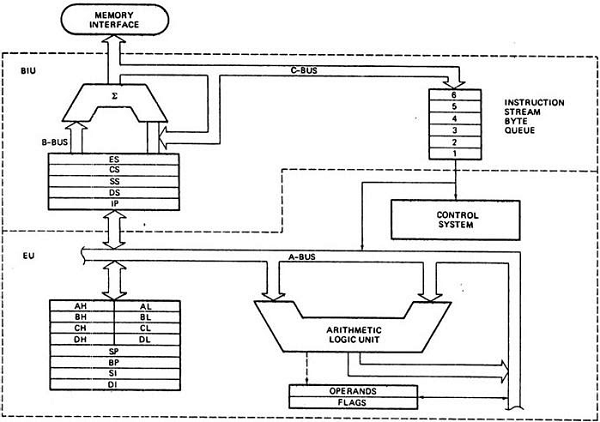
\includegraphics[width=12cm]{figures/8086-architecture.jpg}
    \caption{Kiến trúc của 8086}
\end{figure}

\begin{figure}[H]
    \centering
    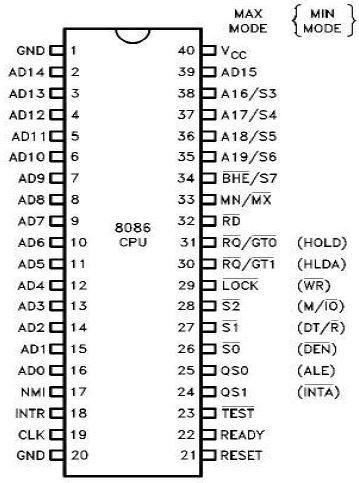
\includegraphics[width=6cm]{figures/8086-pins.jpg}
    \caption{Các chân của 8086}
\end{figure}

Các chân của 8086 ở chế độ Min bao gồm: 
\begin{itemize}
    \item Nguồn: Sử dụng ngồn 5V DC với chân nguồn tại chân 40, chân đất tại chân 1 và 20. 
    \item Tín hiệu clock: chân 19. 
    \item Địa chỉ / Dữ liệu: AD0-AD15. 
    \item Địa chỉ / Trạng thái: A16-A19/S3-S6.
    \item Tín hiệu đọc: Chân 32. 
    \item Tín hiệu sẵn sàng: Chân 22. 
    \item Tín hiệu khởi động vi xử lý: Chân 21.
    \item Tín hiệu báo ngắt: Chân 18. 
    \item Tín hiệu ngắt không che được: Chân 17. 
    \item Tín hiệu kiểm tra: Chân 23. CPU đợi nếu tín hiệu này là cao. 
    \item Tín hiệu phân biệt Minimum / Maximum: Chân 33. 
    \item Tín hiệu chấp nhận ngắt: Chân 24. 
    \item Tín hiệu chốt địa chỉ: Chân 25. 
    \item Tín hiệu chỉ định hướng của dữ liệu: Chân 27. 
    \item Tín hiệu chỉ định bộ nhớ / vào ra: Chân 28. 
    \item Tín hiệu ghi: Chân 29. 

\end{itemize}

\end{document}
